30. $\cfrac{(x-1)^2(x^2-x-2)}{x^2+3x+2}\geqslant0\Leftrightarrow\cfrac{(x-1)^2(x-2)(x+1)}{(x+2)(x+1)}\geqslant0.$
Применив метод интервалов, найдём ответ:
\begin{figure}[ht!]
\center{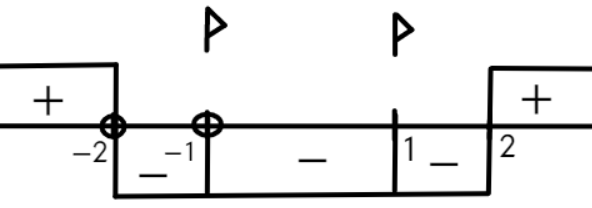
\includegraphics[scale=0.35]{int30.png}}
\end{figure}
$x\in(-\infty;-2)\cup\{1\}\cup[2;+\infty).$\\
